\documentclass[tikz]{standalone}
\usetikzlibrary{shapes.geometric, arrows,fit, shapes.multipart, quotes}
\usetikzlibrary{positioning}
\tikzstyle{box} = [draw=black, fill=gray!20, very thick, rectangle, rounded corners, inner sep=5pt, font=\footnotesize]
\tikzstyle{fancytitle} = [fill=black, text=white, font=\footnotesize]
\tikzset{tree node/.style={draw,circle,line width=0.5pt,minimum size=1cm}}
\tikzset{tree dot/.style={draw,circle,fill,inner sep=0pt,minimum size=3pt}}
\tikzset{tree line/.style={line width=.5pt, color=gray}}
\tikzset{tree dotted/.style={line width=.5pt, color=gray,dotted}}
\tikzstyle{arrow} = [thick,->,>=stealth]
\tikzset{every edge quotes/.style =
	{ fill = white,
		sloped,
		execute at begin node = $,
		execute at end node   = $  }}
\begin{document}
	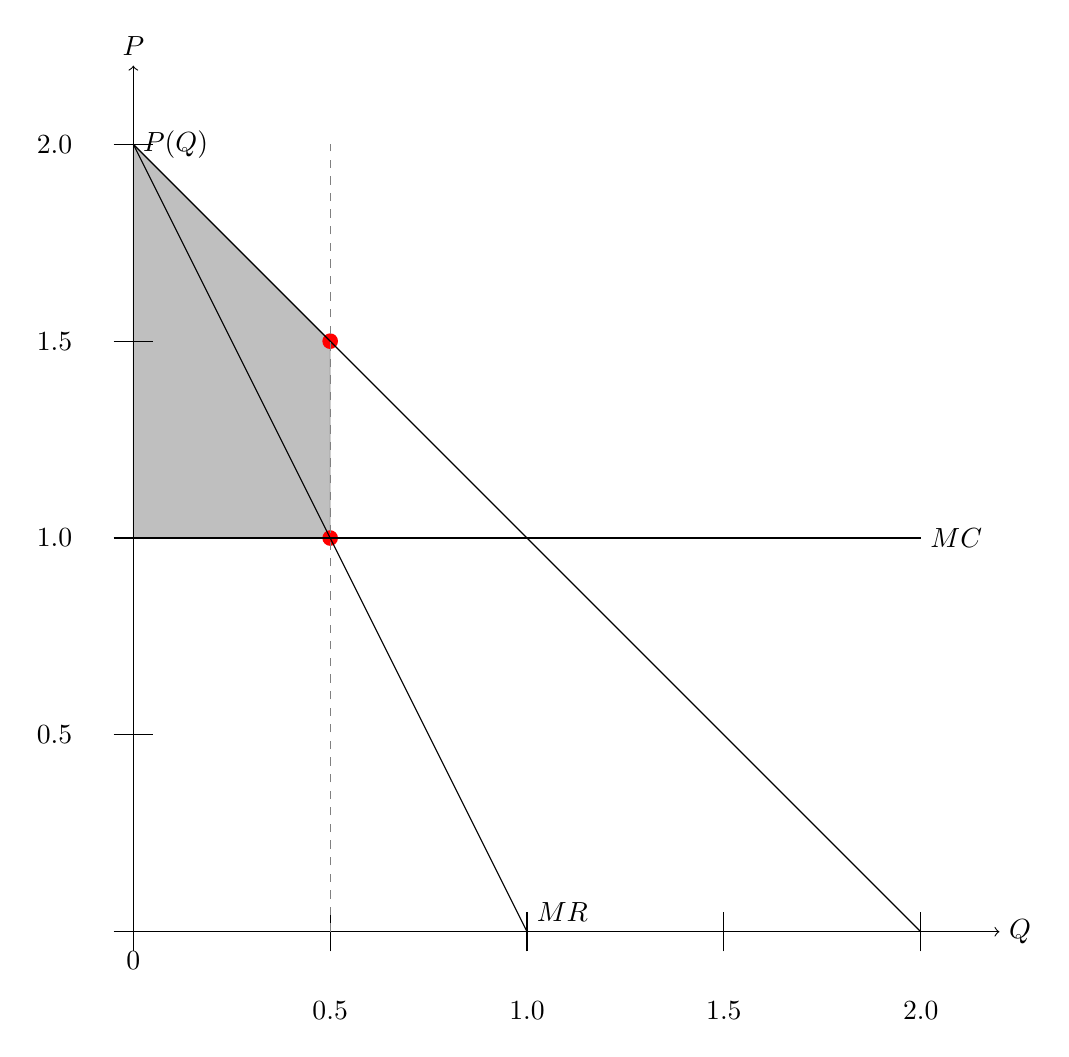
\begin{tikzpicture}[domain=0:2, scale=5]		
		\filldraw[color=gray, opacity = 0.5] (0,1) -- (0,2)  -- (0.5,1.5) -- (0.5,1);		
		%Achsen mit Beschriftung
		\draw[->] (0,0) -- (2.2,0) node[right] {$Q$};
		\draw[->] (0,0) -- (0,2.2) node[above] {$P$};
		
		%Skalierung der Ordinate
		\draw (0,-0.05)--(0,0.05);
		\node[below] at (0,-0.025) {0};
		\draw (0.5,-0.05)--(0.5,0.05);
		\draw (1,-0.05)--(1,0.05);
		\draw (1.5,-0.05)--(1.5,0.05);
		\draw (2,-0.05)--(2,0.05);
		
		\node at (0.5,-0.2){$0.5$};
		\node at (1,-0.2){$1.0$};
		\node at (1.5,-0.2){$1.5$};
		\node at (2,-0.2){$2.0$};
		
		%Skalierung der Abzisse
		\draw (-0.05,0)--(0.05,0);
		\draw (-0.05,0.5)--(0.05,0.5);
		\draw (-0.05,1)--(0.05,1);
		\draw (-0.05,1.5)--(0.05,1.5);
		\draw (-0.05,2)--(0.05,2);
		
		\node at (-0.2,0.5){$0.5$};
		\node at (-0.2,1){$1.0$};
		\node at (-0.2,1.5){$1.5$};
		\node at (-0.2,2){$2.0$};
		
		%punkte mit beschr. 
		\node at (0.5,1.0)[circle,fill=red,inner sep=2pt]{};
		\node at (0.5,1.5)[circle,fill=red,inner sep=2pt]{};
		
		%curves
		\draw (2,0)--(0,2) node[right] {$P(Q)$};
		\draw (0,1)--(2,1) node[right] {$MC$};
		\draw (0,2)--(1,0) node[above right] {$MR$};
		\draw [dashed, color=gray] (0.5,0) -- (0.5,2);
	\end{tikzpicture}
\end{document}